\chapter{Methodology}
\label{sec:problem}

% TODO: Page 38 of Improving Sequential Decision Making in Human-In-The-Loop Systems

% \begin{enumerate}
%     \item How to get transition and observation probabilities? Am I correct that these need to be given by Florian's model? How would this ever be known in the case of learning with real human drivers?
%     \item Is the Markov assumption satisfied even though the driver's attentiveness does not depend on the previous state and action?
%     \item What is known a priori?
%     \begin{itemize}
%         \item human's current action (assumption: no, for performance reasons)
%         \item reward function
%     \end{itemize}
% \end{enumerate}

\section{Lane keeping with a human in the loop as a POMDP}

% TODO: Add state estimator + policy to agent? 
% See (POMDP definition) Planning and acting in partially observable stochastic domains)
\begin{figure}[ht]
    \centerfloat
    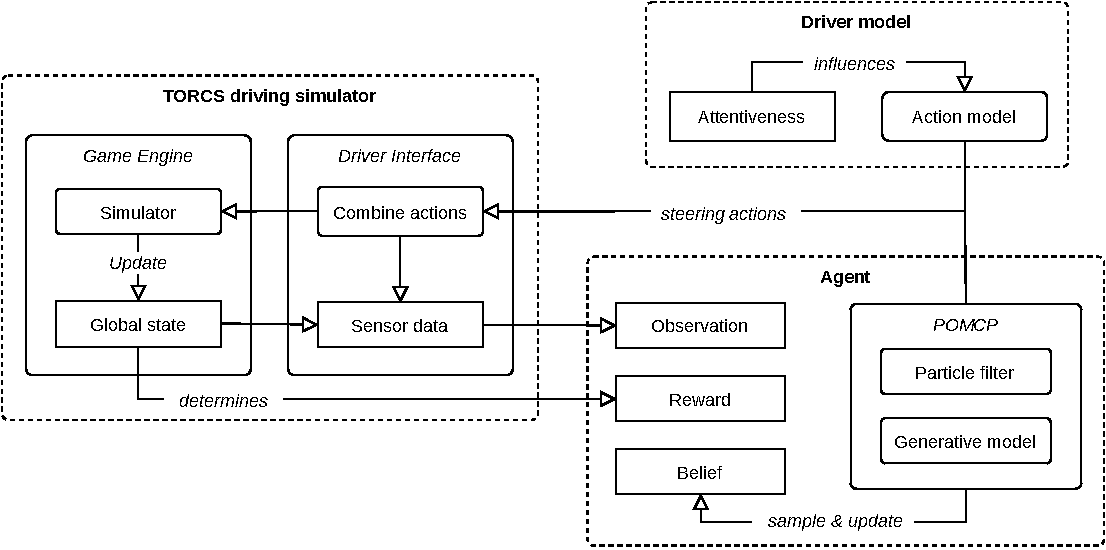
\includegraphics[width=1.2\linewidth]{figures/Components.pdf}
    \caption{Solution approach overview}
    \label{fig:overview}
\end{figure}

% TODO: Add: The agent can only recognize a state change of the driver after the driver has performed the first action in this state. This is because there are no observable clues about the duration of the driver's attentiveness and distraction.

\subsection{Driving simulator TORCS}

\subsubsection{State}

% TODO: Define terminal state

The tracks will be round courses. Thus, there is no terminal state if everything goes well. If the car reaches an off-track position, however, the car is reset to be in the initial starting position again.\\

\begin{tabularx}{\textwidth}{@{}p{0.18\textwidth}>{\centering}p{0.22\textwidth}X@{}}
\toprule
\textbf{Name}           & \textbf{Measurement}          & \textbf{Description}                                           \\ \midrule

Gear \newline \textbf{(constant)} & \{$-1$, $0$, $1$,  \dots, $6$\} & Distance of the car from the start line along the track line. \textbf{Neither the human driver nor the agent can directly influence this with their actions.} \\ \midrule

RPM \newline \textbf{(constant)} & [0, $+\inf$) & Number of engine rotations per minute. \textbf{Neither the human driver nor the agent can directly influence this with their actions.} \\ \midrule

Speed \newline \textbf{(constant)}  & ($-\inf$, $+\inf$) (km/h) & Speed along the longitudinal axis of the car. \textbf{Neither the human driver nor the agent can directly influence this with their actions.} \\ \midrule

% Lift \newline \textbf{(constant)} & ($-\inf$, $+\inf$) (km/h) & Speed along the vertical axis of the car. Will be zero as we use completely flat terrain. \textbf{Neither the human driver nor the agent can directly influence this with their actions.} \\ \midrule

Side force & ($-\inf$, $+\inf$) (km/h) & Speed along the transverse axis of the car. This is directly influenced by the steering actions of both human driver and agent. \\ \midrule

Distance from start & [0, $+\inf$) (m) & Distance of the car from the start line along the track line. \\ \midrule

Angle          & [$-\pi$, $+\pi$] (rad) & Angle between car direction and track axis direction.  \\ \midrule

Lane position & ($-\inf$, $+\inf$)     & Horizontal distance between the car and the track axis. $0$ when the car is on the axis, $+1$ if the car is on the left edge of the track, and $-1$ if the car is on the right edge of the track. Greater numbers than $+1$ or smaller numbers than $-1$ indicate that the car is off-track. \\ \midrule

Driver attention & True / False & Whether the human driver is attentive or distracted.  \\ \bottomrule

\end{tabularx}

\subsubsection{Actions}

\begin{tabularx}{\textwidth}{@{}p{0.18\textwidth}>{\centering}p{0.22\textwidth}X@{}}
\toprule
\textbf{Name}           & \textbf{Measurement}          & \textbf{Description}\\ \midrule

\multicolumn{3}{@{}>{\centering}p{\linewidth}@{}}{\textit{In our simplified scenario, both the human driver and the agent can not accelerate, brake or switch gears.}} \\ \midrule

Steering         & [$-2$, $+2$] & The input to the car is generated by combining the agent's action with the human's steering action (see equation~\ref{eq:steering}). For the car,  $-1$ means full right (159 degrees) and $+1$ means full left (21 degrees). A value greater than +1 or lower than -1 can effectively reverse an opposite action of the human driver. \\ \bottomrule
\end{tabularx}\\\\

\noindent The human driver and the agent share control of the steering wheel. The speed of the car is fixed and cannot be altered; neither by human driver nor agent. The steering input of the driver $\mathcal{A}_{steer}^{driver}$ and agent $\mathcal{A}_{steer}^{agent}$ are combined to ${A}_{steer} \in [-1, +1]$ using equation~\ref{eq:steering}.

The agent needs to be able to fully counteract a distracted driver's actions. In the extreme case, while the car is in a curve, a distracted driver could steer into the opposite direction of the trajectory of the lane center. Thus, the car would not only diverge from the lane center but would even get off the road completely. The agent thus needs to reverse the driver's action in order to keep the car centered in the lane and follow the road curve. Therefore, we define the range for the agent's steering action as follows: $\mathcal{A}_{steer}^{agent} \in [-2, +2]$.

\begin{equation}
    \mathcal{A}_{\textrm{steer}} = \min(\, -1, \, \max(\, 1, \, (\mathcal{A}_{\textrm{steer}}^{\textrm{driver}} + \mathcal{A}_{\textrm{steer}}^{\textrm{agent}})\,)\,)
    \label{eq:steering}
\end{equation}

\subsubsection{Observations}
\label{sec:observations}

\begin{figure}[ht]
    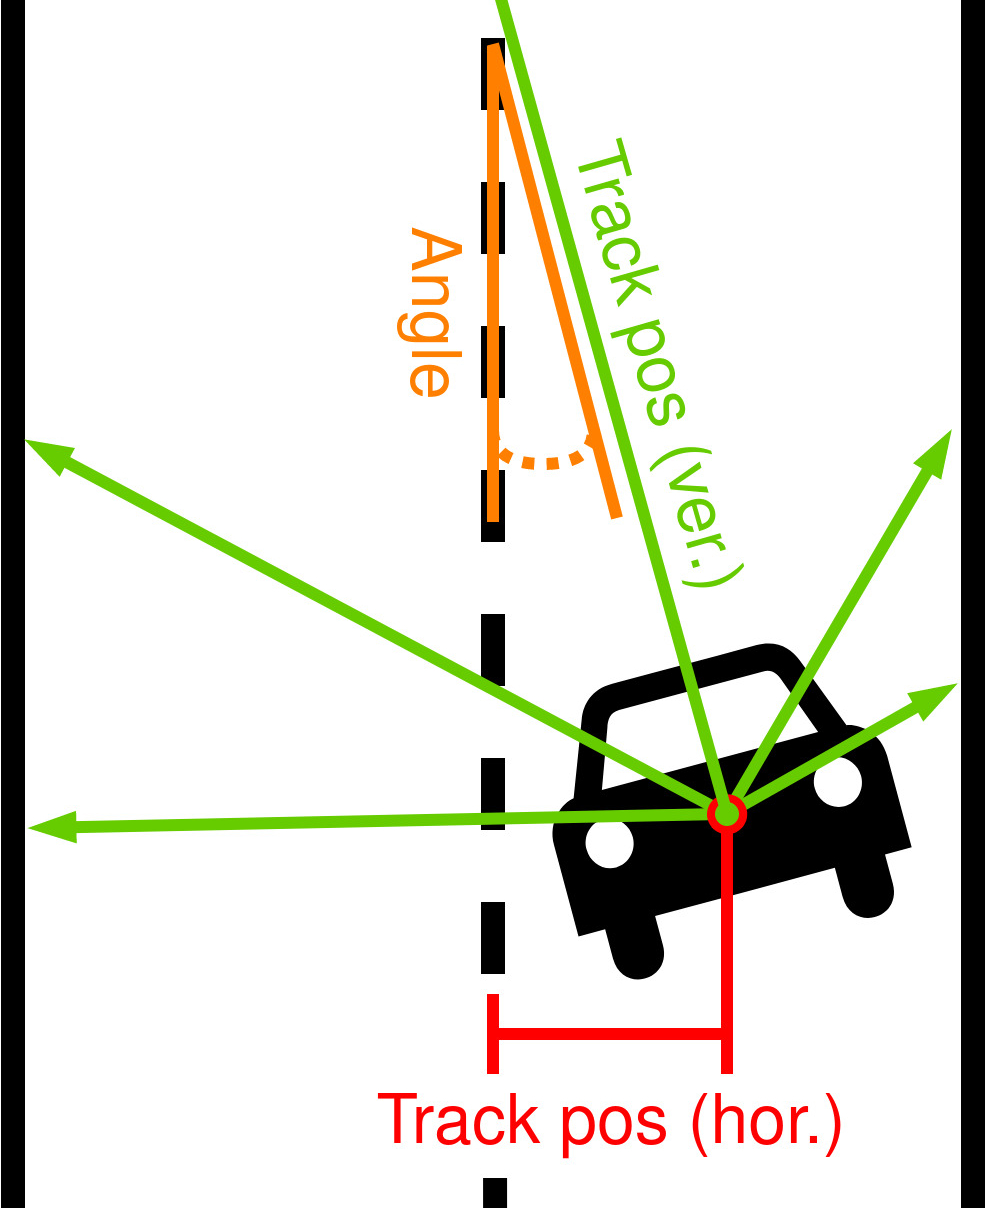
\includegraphics[width=0.3\linewidth]{figures/Observations.jpg}
    \centering
    \caption{Main environment observations}
    \label{fig:observations}
\end{figure}


\begin{tabularx}{\textwidth}{@{}p{0.18\textwidth}>{\centering}p{0.22\textwidth}X@{}}
\toprule
\textbf{Name}           & \textbf{Measurement}          & \textbf{Description}   \\ \midrule

\multicolumn{3}{@{}>{\centering}p{\linewidth}@{}}{\textit{Constant state parameters are not observed as they do not influence learning.} \textbf{The observations are not noisy.}} \\ \midrule

Angle          & [$-\pi$, $+\pi$] (rad) & Angle between car direction and track axis direction  \\ \midrule

Side force & ($-\inf$, $+\inf$) (km/h) & Speed along the transverse axis of the car. This is directly influenced by the steering actions of both human driver and agent. \\ \midrule

Track position (horizontal) & ($-\inf$, $+\inf$)     & Horizontal distance between the car and the track axis. $0$ when the car is on the axis, $+1$ if the car is on the left edge of the track, and $-1$ if the car is on the right edge of the track. Greater numbers than $+1$ or smaller numbers than $-1$ indicate that the car is off-track.  \\ \midrule

Track position (vertical)  & [$0$,$200$] (m) & Vector of 5 range finder sensors (of 19 available in TORCS). The range finders serve as lookahead by returning the distance between the car and the track edge in a given forward angle between $-90$ and $+90$ degrees with respect to the car axis. \\ \midrule 

Driver steering (last time step) & [$-1$, $+1$]  & The agent perceives the last input of the human. This is not the action of the human in the next but in the last time step. The agent does not know which action the human is going to choose simultaneous to its own action. $-1$ means full right (159 degrees) and $+1$ means full left (21 degrees).  \\ \bottomrule
\end{tabularx}

\subsection{Driver model}
\label{sec:driver_model}

The driver model is simplistic. If the driver is attentive, its actions are optimal. The driver model returns the action that steers the car as close to the center of the lane as possible. In this case, the agent should not interfere. However, if a distracted driver is modeled, the driver just repeats the last action it performed while being attentive. This can have the effect of the driver's action to overshoot with the car diverging from the center of the lane. Following, the agent has to identify distracted driving and counteract.

When the driver model is initialized, it is randomly set to be attentive or distracted. The driver stays in this state for a randomly chosen discrete time period between ten and 60 seconds for an attentive state and between two and six seconds for a distracted state. After the chosen time period, the state of attentiveness switches; a previously attentive driver becomes distracted, and a previously distracted driver becomes attentive. The process repeats until the experiment is over.

\subsubsection{Simple driver model}


\subsubsection{Steering over-correction}


\subsubsection{Steering over-correction and noise}

\subsection{Reward}

The overall goal for the agent is to only assist the driver in keeping the car centered in its lane. Therefore, this is the main source of reward for the agent. The more centered the car is at a certain time step, the more reward $r$ is received. However, the agent is supposed to leave the human driver with as much autonomy as possible. Thus, any intervention by the agent is penalized. Minor smooth interventions are generally preferred over large abrupt steering actions. Accordingly, the penalty is (exponentially) dependent on the intensity of the agent's action. The general assumption is that an attentive driver performs better in keeping the car centered than an inattentive driver. The agent has to predict whether a driver is attentive or not in order to choose its actions correctly. An incorrect prediction of the driver's actions will lead to overshooting and thus be negatively reflected in the reward for keeping the car centered. Lastly, the car is never supposed to leave the lane. Consequently, leaving the lane is highly penalized.


%For this reason, the penalty intensity is linked to the current distance of the car to the lane center; the higher the distance, the lower the agent's intervention penalty. On the other hand, 

% TODO: Add smoothing?

% \begin{equation}
%     \mathcal{R} = \mathcal{R}_{\textrm{center}} - \mathcal{P}_{\textrm{act position}} - \mathcal{P}_{\textrm{act intensity}} - \mathcal{P}_{\textrm{off-lane}}
% \end{equation}
\begin{equation*}
    \mathcal{R} = \mathcal{R}_{\textrm{center}} - \mathcal{P}_{\textrm{act intensity}} - \mathcal{P}_{\textrm{off-lane}}
\end{equation*}
\begin{equation*}
    \mathcal{R}_{\textrm{center}} = 
    \begin{cases}
        r - r * |Pos_{hor}| & \text{if} \quad |Pos_{hor}| \leq 1 \\
        0 & \text{if} \quad \text{off-lane}
    \end{cases}
\end{equation*}
% \begin{equation}
%     \mathcal{P}_{\textrm{act position}} = 
%     \begin{cases}
%         p_{\textrm{pos}} - p_{\textrm{pos}} * |Pos_{hor}| & \text{if} \quad |Pos_{hor}| \leq 1 \text{ and } \mathcal{A}_{\textrm{steer}}^{\textrm{agent}} \neq 0 \\
%         0 & \text{if} \quad \text{off-lane or no steering action}
%     \end{cases}
% \end{equation}
\begin{equation*}
    \mathcal{P}_{\textrm{act intensity}} = |\mathcal{A}_{\textrm{steer}}| ^ {p_{\textrm{int}}}
\end{equation*}
\begin{equation*}
    \mathcal{P}_{\textrm{off-lane}} = 
    \begin{cases}
        p_{\textrm{off}} & \text{if} \quad |Pos_{hor}| > 1 \\
        0 & \text{if} \quad |Pos_{hor}| \leq 1
    \end{cases}
\end{equation*}

\section{Solution approach using the POMCP algorithm}
\subsection{Discretization}
\label{sec:discretization}

\begin{figure}[htbp]
    \centering
    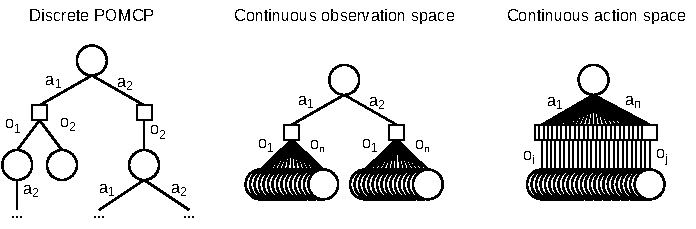
\includegraphics[width=0.8\textwidth]{figures/pomcp_continuous.pdf}
\end{figure}

% Solving continuous POMDPs
% See (POMDP, POMCP, Thesis) Towards Human-Like Prediction and Decision-Makingfor Automated Vehicles in Highway Scenarios

% POMCP tree for a discrete POMDP (left), and for a POMDP with a
% continuous observation space (right). Because the observation space is continuous,
% each simulation creates a new observation node and the tree cannot extend deeper.

% Why do we have to discretize with POMCP?
% See (POMDP, Continuous, POMCPOW, POMCP-DOW, DPW, Thesis) SAFETY AND EFFICIENCY IN AUTONOMOUS VEHICLES THROUGH PLANNING WITH UNCERTAINTY

\subsection{General POMCP definition}
\label{sec:pomcp}

% explain: 
% - Planning versus learning
% - How POMCP breaks the curse of dimensionality with Monte-Carlo sampling
% - Belief and blief update

% Particle filter belief update:
% See (POMDP, Thesis) Tactical Decision-Making forHighway Driving

% TODO: Replace planning time with number of searches
% TODO: Add select random
% TODO: Fix arrow for h = hao, s=s' (Use two diagonal arrows)
% TODO: Add caption
% TODO: Mark rollout and search phase as in the original paper
\begin{figure}[htbp]
    \centerfloat
    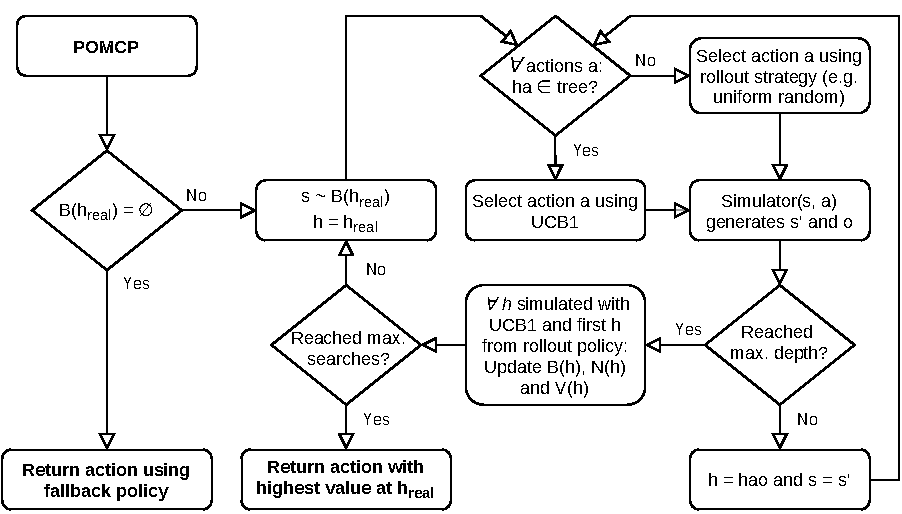
\includegraphics[width=1.2\textwidth]{figures/POMCP.pdf}
\end{figure}

\Gls{pomcp} constructs a search tree with nodes representing histories $h$ of actions and observations. At each node, $N(h)$ stores the number of times the represented history $h$ has been encountered, $V(h)$ is the node's value that is approximated by the average return of simulations starting at history $h$, and $B(h)$ represents the node's belief over the real environment's state. $B(h)$ is a collection of potential states where the likelihood of each state is given by the relative number of times it is included in the collection.

If the belief at the node representing $h_{real}$ is empty, an initial state distribution $I$ is used to sample a start state $s$ for the search. Otherwise, $B(h_{real})$ is utilized. The search tree is then searched in two stages. First, in the case that the search tree already contains child nodes for all actions at the current history, UCB1 is used for the action selection. Exploration is achieved by increasing the value of rarely-tried actions by an exploration bonus. Second, when the tree is missing a node for a potential action at the current history, a rollout policy is used to select actions. In the most simple case, this means choosing uniformly random over the action space. In either case, the selected action is executed on the start state $s$, leading to a successive state $s'$, observation $o$, and reward $r$. The process is repeated with resulting successive states until a maximum depth of the tree is reached. Afterwards, the beliefs, counts, and values are updated at all nodes for the histories resulting from the UCB1 action selection, and the node for the first history resulting from the rollout policy. The belief is updated by adding the successive states $s'$ from the simulator to the collections $B(ho)$ in the nodes. If the maximum planning time has not yet been reached, another start state is sampled and the whole process repeats. When the time runs out, the action $a_{best}$ with the highest value at the current history $h_{real}$ is returned. After this action is executed in the real environment, with an observation $o_{last}$ the tree can be pruned. Only the nodes from history $h_{real}a_{best}o_{last}$ onward stay relevant as all other histories are rendered impossible.

% TODO: Add particles as a construct (Or change particles everywhere else to "state in the belief")
% See Algorithms for decision making book

% One common approach is to use a particle filter, which represents the belief state as a collection of states. 10 Each state in the approximate belief is called a particle.

\subsection{Particle deprivation and particle injection}
\label{sec:particle_deprivation}

Particle filter approaches, POMCP included, can fail due to a phenomenon called particle deprivation. Because of the random nature of the process, the belief can sometimes converge towards a state that is far from the environment's true state. Particles that differ from the converged state have a low probability to be selected while sampling (low relative count). Hence, with each iteration, they become scarcer until they are completely erased from the belief. At this point, the agent is sure to be in an erroreous state and cannot recover anymore. Particle injection (also called particle reinvigoration) is a method to counteract this problem by introducing a number of random particles to the belief at each iteration \parencite{decision_making_book}. While this reduces the accuracy of the belief, it prevents its complete convergence towards a wrong state. 

Particle injection is used to increase the variance of the belief about the driver model state. Only observable information is used. Concretely, particle injection is implemented by adding driver model states with a random number of remaining actions and the same action as the one that was last observed. The number of remaining actions can be lower than the minimum defined in Section~\ref{sec:driver_model} because this limit is only intended for initial sampling and the true remaining number of driver actions in a particular state might be lower after having performed actions already. Like in the original POMCP paper, the amount of transformed particles that are added before each planning step is $1/16$ of the number of searches. The particles can be added during policy execution, and therefore, do not influence planning time.

% Use term posterior probability distribution? We can only add particles after making an observation so that we can verify that the potential particles to add match this belief.


\subsection{Action selection and preferred actions}
\label{sec:action_selection}

% TODO: Just say the agent does not act anymore when losing track with the belief instead of using uniformly random action selection? Makes more sense.

% This is strongly related to the particle deprivation problem described in Section~\ref{sec:particle_deprivation}. When the driver is in a distracted or attentive state, any number of remaining actions in this state below the maximum number (see Section~\ref{sec:driver_model}) could be valid and can therefore be part of the driver model states in the belief. In successive iterations, particles that represent drivers switching their state earlier than the true driver, and therefore change their steering behavior, are ruled out and removed from the belief. Thereby, after some iterations, driver model states that have the same or more remaining actions than the true state dominate the belief.

% preferred actions = domain knowledge

\subsection{Generative model}
\label{sec:gen_model}

